\setlength{\abovedisplayskip}{0pt}
\setlength{\belowdisplayskip}{0pt}
\setlength{\abovedisplayshortskip}{0pt}
\setlength{\belowdisplayshortskip}{0pt}

\chapter{Background}
\label{chap:background}
\textit{In this chapter, we introduce the foundation knowledge of the thesis, including the Blockchain Technology, Cryptography, and Hierarchical Deterministic Wallet (HD wallet)}

\minitoc

\section{Blockchain Technology}

\subsection{History and Definition}

% Blockchains are immutable digital ledger systems implemented in a distributed fashion (i.e., without a central repository) and usually without a central authority.
% The definition of blockchain was introduced to the world by a person (or a group of people) under the name Satoshi Nakamoto on October 31, 2008 \cite{Bitcoin:Bitcoin}.
% It was applied to enable the emergence of a "purely peer-to-peer (no financial institution or third party) electronic cash" named Bitcoin where transactions take place in a distributed system.
% In fact, Satoshi did not invent blockchain, and Bitcoin blockchain is not the first chain that ever created.
% Back in 1991, cryptographers Stuart Haber and Scott Stornetta published a whitepaper "How to Time-Stamp a Digital Document" in the Journal of Cryptography \cite{DBLP:journals/joc/HaberS91}.
% Their goal is to digital time-stamping of documents so that it is infeasible for a user either to back-date or to a forward-date digital document, even with the collusion of a time-stamping service.
% The technology is called a blockchain because the distributed electronic ledger stores items of data in time-stamped digital groups called blocks. Each block includes an alphanumeric code called a "hash" summing up its data. The hash of each completed block also appears in the next one in the chain, which means that to alter one block you would have to alter all the ones connected to it. These cryptographic dominos function together to protect against tampering or fraud.
% Base on this theory, the longest-running blockchain, started in 1995, also by Haber and Stornetta, publishes the weekly summary hash value every week in the New York Times (\autoref{fig:first_blockchain}) and still running strong today.

% \begin{figure}[ht!]
%   \centering
%   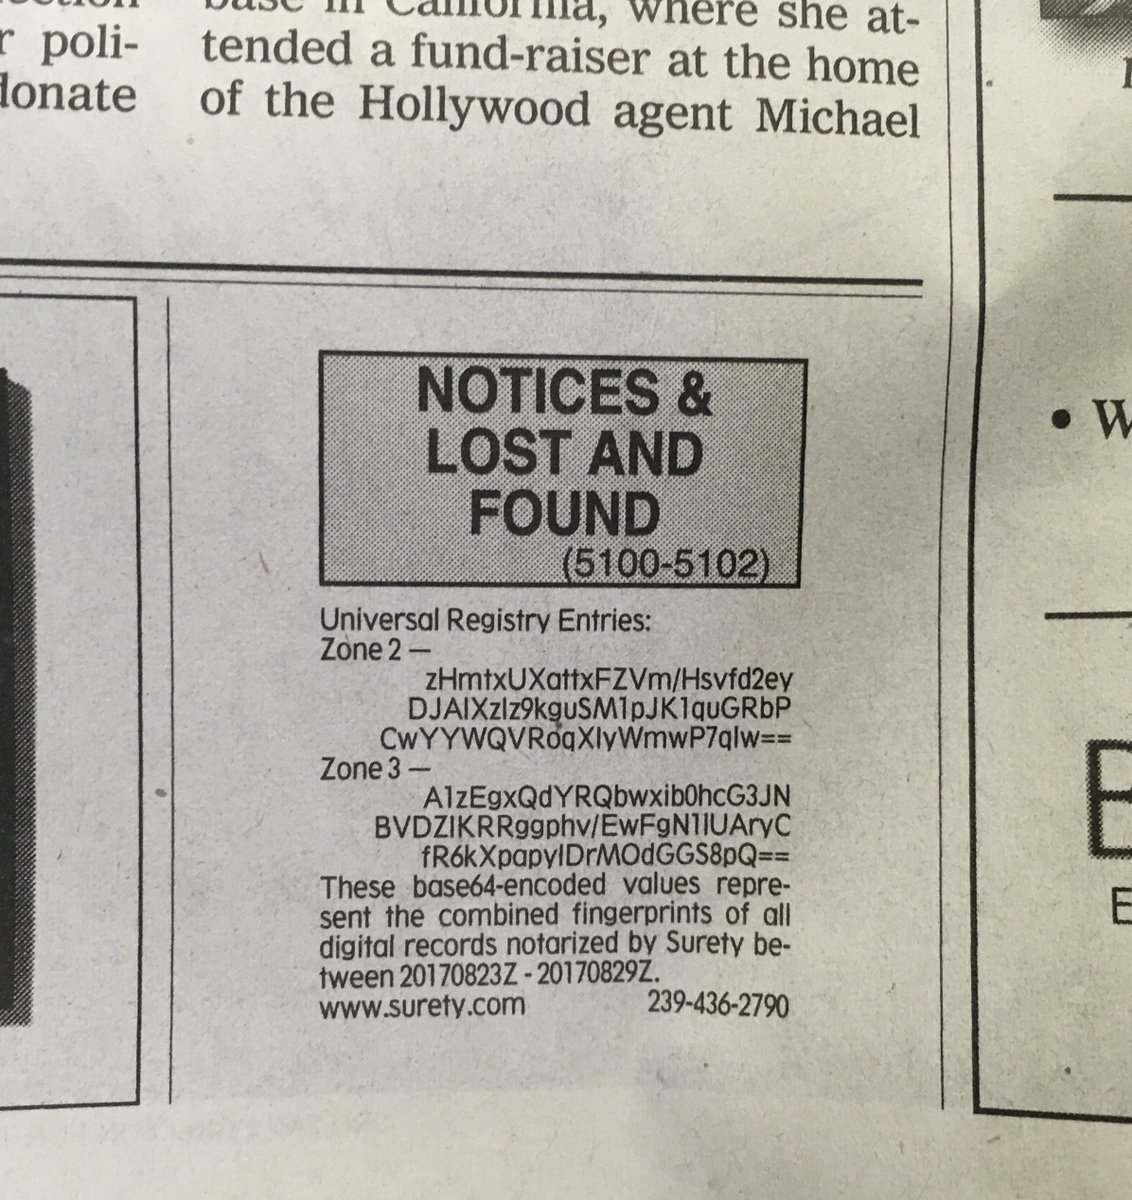
\includegraphics[width=.35\textwidth]{images/Widely_Witnessed_Values.jpg}
%   \caption[Widely-Witnessed Values of Surety, a weekly summary (hash) of documents]{Weekly summary hash value in The New York Times}
%   \label{fig:first_blockchain}
% \end{figure}

% % The math behind blockchain and its complex system architecture make it challenging to understand. 
% But the word "blockchain" or "block" and "chain" wasn't use back then.
% Only when it was known in Satoshi Nakamoto's Bitcoin paper does the term of "chain" of "blocks" become a representaion for this technology.
% Later people combined the one-word "blockchain" in mainstream media publications such as Fortune, Forbes, and the Huffington Post as the technology gained greater interest and use \cite{blockchain:meaning}.
% The community use that word for Nakamoto's invention.
% Bound to the emergence of Bitcoin and cryptocurrency, a concise description of blockchain technology is provided by NIST:

% \begin{quote} 
%   Blockchains are distributed digital ledgers of cryptographically signed transactions that are grouped into blocks. Each block is cryptographically linked to the previous one (making it tamper evident) after validation and undergoing a consensus decision. As new blocks are added, older blocks become more difficult to modify (creating tamper resistance). New blocks are replicated across copies of the ledger within the network, and any conflicts are resolved automatically using established rules \cite{BlkchainOverview}.
% \end{quote}

% Blockchain technology comes handy in a wide range of areas - both ​financial and non-financial​.
% Non-Financial application opportunities are endless.
% We can envision putting proof of the existence of all legal documents, health records, and loyalty payments in the music industry, notary, private securities and marriage licenses in the blockchain.
% By storing the fingerprint of the digital asset instead of storing the digital asset itself, the anonymity or privacy objective can be achieved.
% For the sake of our thesis, we will mainly focus on the original and surely the most popular application of blockchains - Cryptocurrency.

% Cryptocurrencies are digital currencies that use blockchain technology to made reality and still running strong today (\autoref{fig:first_blockchain}).
% A cryptocurrency can be used as a digital form of cash that can be used to buy goods and services.
% It can be bought using one of several digital wallets or trading platforms, then digitally transferred upon purchase of an item, with the blockchain recording the transaction and the new owner.
% The appeal of cryptocurrencies is that everything is recorded in a public ledger and secured using cryptography, making an irrefutable, timestamped, and secure record of every payment.
% The ledger displays user account balances and inter-user payments in a “currency” defined by the ledger itself and not necessarily in one of the traditional currencies.
% Nevertheless, cryptocurrency may be traded on the stock exchange and exchanged for traditional money, which makes it hard to distinguish between traditional currency and cryptocurrency and as official vs. non-official currency.
% The most widely recognized cryptocurrency system is Bitcoin.

% We believe the "magic" that brings the above concept of digital currencies to reality, beside blockchain technology, is Nakamoto's proof-of-work consensus model.  

% \subsection{Blockchain Characteristics and Generations}

% Blockchain network can be:
% \begin{itemize}
%   \item \emph{Permissioned network}, where users publishing blocks must be authorized by some authority (be it centralized or decentralized).
%         Users of blockchain have to trust that entity or user who published blocks.
%         Permissioned blockchain networks may thus allow anyone to read the blockchain or they may restrict read access to authorized individuals. This maybe used by organizations that need more control over their blockchain.
%         Some permissioned blockchain networks support the ability to selectively reveal transaction information based on a blockchain network users identity or credentials.
%         Some of famous permissioned blockchain applications are \href{https://ripple.com/}{Ripple}, which enables interbank transactions, or \href{https://sovrin.org/}{Sovrin}, which is managed by financial institutions and is seeking to build a global decentralized identity system.

%   \item \emph{Permissionless network}, where service providers are not fixed and, in principle, anyone can start operating the service.
%         For example, Bitcoin and the early versions of \href{https://ethereumclassic.org/}{Ethereum}.

%   \item \emph{Centralized network}, where the ledger is managed as a centralised service by one legal	entity. For example, the \href{https://guardtime.com/}{Guardtime} system.
% \end{itemize}

% % The blockchain is usually stored and managed in the form of a distributed ledger,
% % with multiple parties keeping a copy of the ledger, which then implies the use of a
% % handshake protocol between the components. However, also centralized blockchain
% % system exist. The original and surely the most popular application of blockchains is
% % cryptocurrency, where the ledger displays user account balances and inter-user payments
% % in a “currency” defined by the ledger itself and not necessarily in one of the traditional
% % currencies. Nevertheless, cryptocurrency may be traded on the stock exchange and
% % exchanged for traditional money, which makes it hard to distinguish between traditional
% % currency and cryptocurrency and as official vs. non-official currency. The most widely
% % recognised cryptocurrency system is Bitcoin, which establishes and uses Bitcoins and
% % Satoshis as currency.

% % Most permissionless blockchain systems include an independent cryptocurrency. 
% % The reason for that is that in the absence of an inter-operator contract, there are usually no other incentives to guarantee voluntary management of the Blockchain

% Based on the intended audience, three generations of blockchains can be distinguished:
% \begin{itemize}

%   \item Blockchain 1.0 which includes applications enabling digital cryptocurrency transactions
%   \item Blockchain 2.0 which includes smart contracts and a set of applications extending beyond cryptocurrency transactions
%   \item Blockchain 3.0 which includes applications in areas beyond the previous two versions, such as government, health, science and IoT.

% \end{itemize}

% We are now developing blockchain 2.0 but our thesis just focuses on the cryptocurrency aspect.


% \subsection{Bitcoin blockchain}
% Bitcoin is the first application of blockchain and the most famous digital currency ever.
% As mentioned above, Bitcoin was invented with the publication of a document entitled "Bitcoin: A peer-to-peer electronic cash system" in 2008 by Satoshi Nakamoto \cite{Bitcoin}, mentioned as a purely P2P version of electronic cash would allow online payments to be sent directly from one party to another without going through a financial institution.
% The currency began to use in 2009 when its implementation was released as open-source software.
% The Bitcoin blockchain is considered to be a world-changing technology because in the first time in human history its solved the biggest problem of distributed system: The Byzantine General's Problem \cite{DBLP:journals/toplas/LamportSP82}.
% We will talk about this in the Bitcoin game of theory and incentives section.

% Bitcoin application is one of the permissionless blockchain.
% It utilize well-known computer science mechanisms (linked lists, distributed networking) as well as cryptographic primitives (hashing, digital signatures, public/private keys) mixed with financial concepts (ledgers, games of theory) in high level.
% Base on the problems Bitcoin has solved, we examine by dividing it into 3 components:

% \begin{itemize}
%   \item Secure and prevent tempering the data

%         \begin{quote}
%           \emph{Hashes} -
%           Cryptographic hash functions (CHF) are used for hashing the content of a block, validating the integrity of data, reduce the size of the message or keys, generating a Bitcoin address. We will show detail at Section~\ref{sec:crypto_hash}.
%           Hashing is a method of calculating a relatively unique fixed-size output (called a message digest, or just digest) for an input of nearly any size (e.g., a file, some text, or an image).
%           Even one single bit change of input will result in a completely different output digest.
%           In Bitcoin and most blockchain technologies, SHA-256 (Secure Hash Algorithm with output size of 256 bits) appear the most. Many computer support hardware level for this algorithm.
%           NIST specified this algorithm for SHA-256 in Federal Information Processing Standard (FIPS) 180-4 \cite{DBLP:journals/cryptologia/Dang13} as it passed every properties of a cryptographic hashing.
%           \autoref{fig:example_of_sha-256} is an example of SHA-256.

%           \begin{figure}[ht!]
%             \centering
%             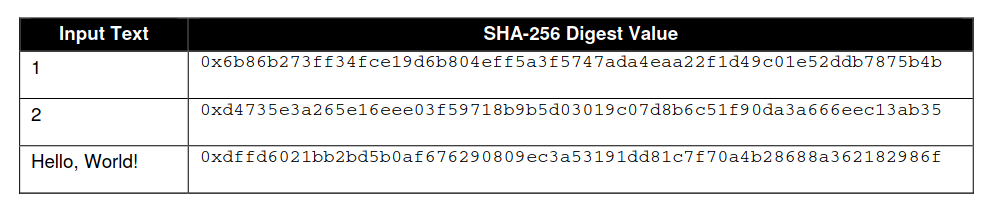
\includegraphics[width=1\textwidth]{images/example_of_sha-256.png}
%             \caption[Example input and output of SHA-256 Digest Value]{Example I/O of SHA-256 Digest Value}
%             \label{fig:example_of_sha-256}
%           \end{figure}

%           \bigbreak

%           \emph{Public/Private Key} -
%           Asymmetric-key cryptography (or public-key cryptography) uses a pair of keys: a public key and a private key that are mathematically related. It could be infeasible to generate one key from the other.
%           The private key is kept secret while the public key can be to everyone, both keys are hold inside user's Wallet, which we present in Section~\ref{sec:hd_wallet}.
%           One can encrypt with a private key and then decrypt with the public key.
%           Alternately, one can encrypt with a public key and then decrypt with a private key.
%           Bitcoin uses asymmetric-key cryptography to digitally sign transactions, verify signatures or in some cases, exchange the key.
%           Asymmetric-key cryptography is discussed in Section~\ref{sec:asymmetric_cryptography}.
%           Figure~\ref{fig:asymmetric_cryptography} briefly show message exchange usage of the asymmetric protocol.

%           \begin{figure}[ht!]
%             \centering
%             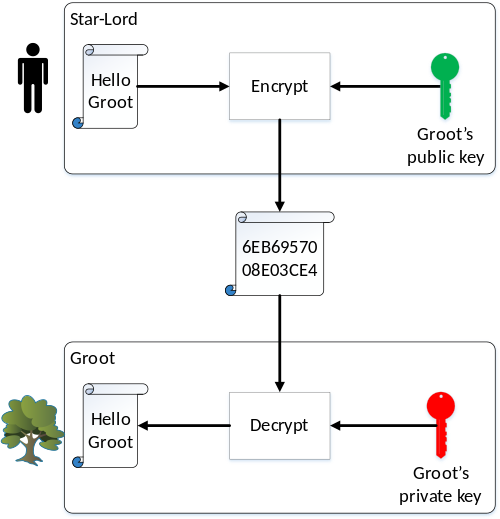
\includegraphics[width=0.4\textwidth]{images/asymmetric_cryptography.png}
%             \caption[An example of concept of Asymmetric-key cryptography]{Sending private message using Asymmetric-key cryptography}
%             \label{fig:asymmetric_cryptography}
%           \end{figure}
%           \bigbreak

%           \emph{Transactions} - Transactions represent transfers of the cryptocurrencies between wallets in the system.
%           A transaction contains input and output. The inputs are usually a list of the digital assets to be transferred.
%           Outputs are	the accounts that will be the recipients of the digital assets along with how much digital asset they will receive.
%           The  output  of  a  transaction  is categorized  by  either  unspent  transaction  output  (UTXO)  or spent  transaction  output  (STXO)
%           All values of in and out cannot be tampered with.

%           \begin{figure}[ht!]
%             \centering
%             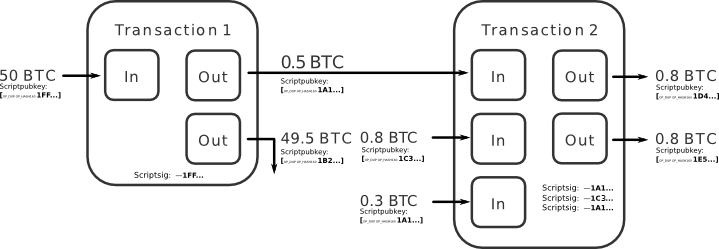
\includegraphics[width=0.7\textwidth]{images/transaction.png}
%             \caption[An example of bitcoin transaction]{An example of bitcoin transaction}
%             \label{fig:transaction}
%           \end{figure}
%           \bigbreak

%           All transactions are broadcast to the network and usually begin to be confirmed within 10-20 minutes, through a process called \emph{mining}.
%           Transactions are typically digitally signed by the sender’s associated private key and can be verified using the associated public key.

%           \bigbreak

%           \emph{Ledgers} -
%           A ledger is a collection of cryptographic transactions.
%           Bitcoin ledgers are distributed, the blockchain holds all accepted transactions within its ledgers. Every user can maintain their own copy of the ledger.
%           Whenever new full nodes join the blockchain network, they reach out to discover other full nodes and request a full copy of the blockchain network’s ledger, making loss or destruction of the ledger difficult.
%           \bigbreak

%           The network utilizes cryptographic mechanisms such as digital signatures and cryptographic hash functions to provide tamper-evident and tamper-resistant ledgers.
%           Due to the public distributed network, the Bitcoin blockchain is harder to attack. There is nothing to steal because everything is distributed. If one individual node got taken down, the network will still be running.
%           If targeting the blockchain itself, the attackers will face resistance from the honest nodes present in the system.
%           \bigbreak

%           \emph{Blocks} -
%           Transactions, after sent to the network (by wallets, web applications, etc.), will be, if accepted, added to a block that is published by a chosen node.
%           Bitcoin blocks include block header and block data.
%           Figure~\ref{fig:block_component} show basic component of a block.
%           Block header contains Height, previous block header’s hash value (prevBlockHash), a hash representation of the block data (usual Merkle tree* hash), a timestamp, size of the block (bits), a \emph{nonce}, etc.
%           The \emph{nonce} value is manipulated by the publishing node to solve the hash puzzle (see Game of theory \ref{item:game_theory})
%           Block data contains a list of transactions and ledger events. Some include other data.
%           \pagebreak

%           \begin{figure}[ht!]
%             \centering
%             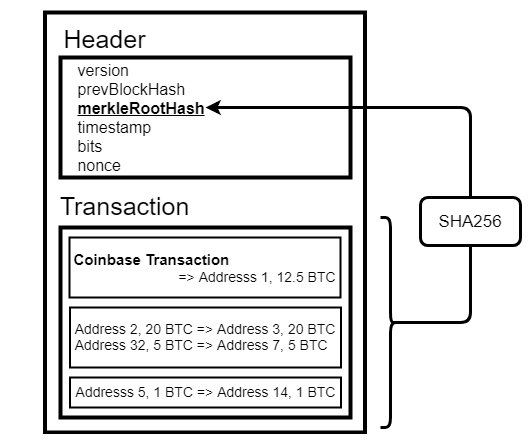
\includegraphics[width=0.6\textwidth]{images/block_component.jpg}
%             \caption[Components of Bitcoin block]{Components of Bitcoin block}
%             \label{fig:block_component}
%           \end{figure}

%           \emph{Chain of Blocks} -
%           Blocks are chained together through each block containing the hash digest of the previous block’s header, thus forming the blockchain.
%           If one of the previous blocks were changed, it would result in a different hash.
%           This makes it possible to easily detect and reject altered blocks

%           \begin{figure}[ht!]
%             \centering
%             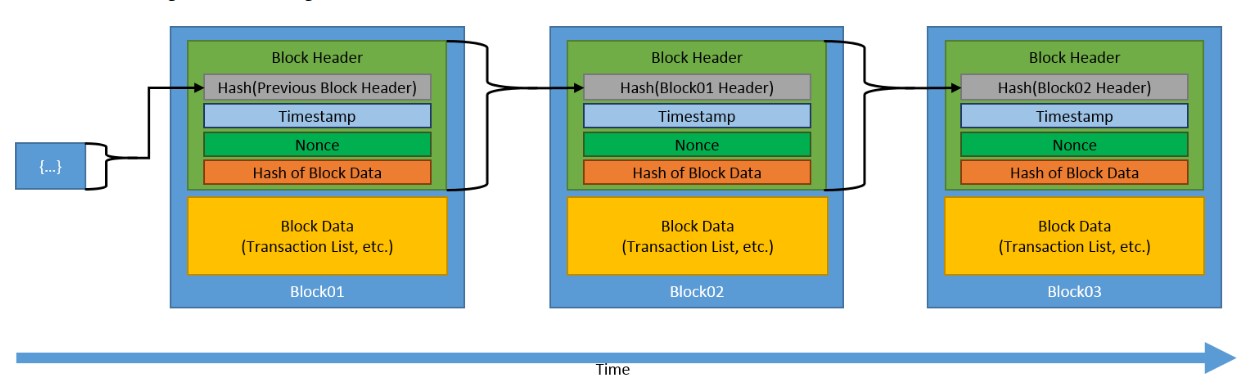
\includegraphics[width=1\textwidth]{images/chain_of_block.png}
%             \caption[Components of Bitcoin block]{Components of Bitcoin block}
%             \label{fig:chain_of_block}
%           \end{figure}

%         \end{quote}

%   \item Game of theory and Incentives
%         \label{item:game_theory}

%         Arthur C. Clarke once wrote, “Any sufficiently advanced technology is indistinguishable from magic”.
%         Clarke’s statement is a perfect representation for the emerging of Bitcoin.
%         Bitcoin blockchain is considered to be a masterpiece of combination of mordern technologies, economics, mathematics, philosophy, and game theory.
%         What make it so special is applying game of theory to solve the The Byzantine General’s Problem \cite{DBLP:journals/toplas/LamportSP82}.

%         Game theory is based on the assumption that all participants are rational actors and are trying to maximize their gains from the game.
%         In the situation of Bitcoin, the problem is how to ensure that all the actors of a decentralized network behave correctly.
%         This is known as The Byzantine General’s Problem \cite{DBLP:journals/toplas/LamportSP82}.
%         How to ensure that all generals will follow the plan? Even if they are located in different places and do not trust each other?
%         This was believed to be the biggest problem of P2P network, impossible to achieve before Satoshi Nakamoto.

%         To make Bitcoin work, Nakamoto invented a model called Proof of Work Consensus Model.
%         In simple words, the proof-of-work involves incrementing the \emph{nonce} in the block that when hashed with SHA-256, the hash begins with a number of zero bits (number of zero bits called the difficulty).
%         User publishes the next block by being the first to solve this puzzle, such users are miners in Bitcoin.
%         Finding a block with a specified difficulty is called mining. When successfully mined a new block, the miner gets some Bitcoin as a reward, this is called \emph{incentive}.
%         The \emph{incentive} help encourage nodes to stay honest.
%         The accepted chain among the system is the longest chain, which has the greatest proof-of-work effort invested in it.
%         If a majority of honest nodes control the power, the honest chain will grow the fastest and outpace any competing chains.
%         Proof-of-work aims to protect the integrity of the ledger by making it hard to modify transactions in "old" entries, as changing a block would also require changing all subsequent (later) blocks.

%   \item Communication Network
%         \begin{quote}
%           Bitcoin blockchain network is peer-to-peer relying on consensus PoW model, where peers (or nodes) are equal right in terms of authority.
%           New nodes can join at any time. The connection establishes over TCP, generally on port 8333, an ad-hoc network with random topology.
%           The system is designed to eliminate third party in certifying transactions in term of trust and reliability.
%           This drives step from a centralized to a decentralized solution.
%           Also, as the nature of decentralized network, it will work even if a single point of network failure.
%           A problem of cryptocurrency is double spending attacks. A malicous user can spend his asset on multiple transactions.
%           For distributed network to accomplish this, all transactions have to be publicly broadcast through the network.
%           The payee needs proof that at the time of each transaction, the majority of nodes agreed it was the first received through consensus agreement.
%           How ever if an attacker is able to control at least 51\% of the has power of the network, they can commit double transaction and verify it.
%           This attack is feasible now since more than 60\% of mining power are located in China.

%         \end{quote}
% \end{itemize}

% \section{HD wallet}
% \label{sec:hd_wallet}

% \subsection{Blockchain wallet}
% A blockchain wallet, sometimes referred as a cryptocurrency wallet or crypto wallet, is a program that allows you to “store”, send and receive digital currencies. Since cryptocurrency doesn’t exist in any physical form, your wallet doesn’t hold any of your coins actually. Instead, it tracks the transactions you made, which is stored in blockchain, and then infers your balance. Thereby, blockchain is an essential component of a blockchain wallet.

% Instead of holding physical coins, a wallet has a public key and a private key. Public key is a long sequence of letters and numbers that forms the wallet address. With this, people can send money to the wallet. It's similar to a bank account number in that it can only be used to send money to an account. Private key is used to access the funds stored in the wallet. With this, people can control the funds tied to that wallet's address. It's a lot like your PIN number in that you should keep it 100\% secret and secure. However, it's worth noting that not all wallets give you sole ownership of your private key, which essentially means that you don't have full control over your coins. As well as storing your public and private keys, crypto wallets interface with the blockchains of various currencies so that you can check your balance and send and receive funds.

% \subsection{Category}

% Now that you know what it is, let’s take a closer look at the five different types of wallets available, each with its own advantages and disadvantages in terms of security, ease of use, convenience and a range of other factors. The most common type of wallet out there, desktop wallets are downloaded and installed on your computer. Easy to set up and maintain, most are available for Windows, Linux and Mac, although some may be limited to a particular operating system. Many cryptocurrencies offer a desktop wallet specifically designed for their coin.

% Desktop wallets provide a relatively high level of security since they’re only accessible from the machine on which they’re installed. The biggest disadvantage is that they also rely on you to keep your computer secure and free of malware, so antivirus and anti-malware software, a strong firewall and a common-sense approach to security are required to keep your coins safe. Most desktop wallets will provide you with a long string of words upon installation. These words are known as your recovery seed or sentence and map with your private key, so it’s important to store them somewhere safe in case your computer dies or you need to format the operating system and re-install your desktop wallet. Some popular desktop wallets: Electrum, Exodus, Copay.

% Mobile wallets are fairly similar to desktop wallets, with the obvious difference being that they run as an app on your smartphone. Mobile wallets feature many of the same advantages and disadvantages as desktop wallets, with your private key stored on your device. Smartphone wallets are often easier to use compared to their desktop counterparts and include the ability to scan other wallet addresses for faster transactions. They also make it simpler to access your coins on the go and use cryptocurrency as part of everyday life. You will need to be extra careful about losing your smartphone, though, because there’s a risk that anyone who has access to your device might also have access to your funds. Choosing an app that allows you to back up your wallet with a 12- or 24-word passphrase is a good idea. Popular mobile wallets: Jaxx, Coinomi, Edge.

% Online wallets (most often provided by exchanges but sometimes offered by third parties) are connected to the Internet and are generally the easiest to set up and use. Most only require an email address and a password to create an account, and web wallets are usually designed to provide a simple and straightforward user experience. The biggest advantages to online wallets are that they can’t be lost and that they’re accessible from any computer with an Internet connection. However, being online is unfortunately also their biggest disadvantage. Because some platforms maintain the wallets of thousands of users, they can become hot targets for hackers. It’s also important to check whether the wallet you choose lets you retain complete control of your private keys or whether they’re owned by the wallet provider. Popular web wallets: blockchain.info, MyEtherWallet, Coinbase.

% Hardware wallets add another layer of security by keeping your private key on a USB stick or specially designed piece of hardware. They allow the user to plug the USB stick into any computer, log in, transact and unplug – so while transactions are carried out online, your private key is stored offline and protected against the risk of hacking. As a result, hardware wallets are widely considered to offer the most secure storage option. The biggest disadvantage of hardware wallets is that they’ll cost you. Prices vary depending on the model you choose, but they generally cost upwards of \$150. You also need to keep the device safe, but if you do lose your hardware wallet, the device itself is PIN-protected and there are usually other protective measures in place to help you recover your funds. Popular hardware wallets: Ledger Nano X, Ledger Nano S, TREZOR, KeepKey.

% Paper wallets take the concept of entirely offline keys used for hardware wallets to the next logical step: simply print out your public and private keys and use that piece of paper as your wallet. As secure as they are, paper wallets are also complex and quite confusing for beginners. They’re typically only used by advanced users who want a high level of security. To transfer money to a paper wallet, you use a software wallet (any of the above mentioned) to send money to the public key printed on the sheet of paper. Most often, this is printed as a QR code for easy scanning. To transfer money from the paper wallet to someone else, you would first need to transfer money to a software wallet (by manually entering the private key into the software), and then transfer money from the software wallet to the recipient as usual. Popular paper wallets: Bitaddress.org, WalletGenerator.net.

% As you’re researching and comparing a range of wallets, you’ll probably come across the terms “hot wallet” and “cold wallet”, or perhaps the concept of “cold storage”. So, what does temperature have to do with crypto storage? A wallet is hot when it's connected to the Internet. Nothing on the Internet is 100\% secure, so funds kept in a hot wallet are always at a slight risk of theft or loss from software bugs or hackers. A wallet is cold when it's safely offline and can't be deliberately or accidentally compromised over the Internet.

% \subsection{HD wallet}

% From economic aspect, the wallet can be custody (required KYC) or non-custody (doesn't required KYC). Since the wallet will interact with a decentralized and transparent ecosystem, obviously the wallet should be non-custody. From key management aspect, we can re-categorize the wallet into three main groups: hardware, software and hybrid. Hardware wallets are not connected to the internet and you have no information about the secret keys whereas software wallets are connected to the internet and store your secret keys. Hybrid is the combination of both hardware and software wallet, that they store your secret keys and are managed by the software. We will develop on a hybrid wallet as we need some information about the secret keys and need to manage the keys.

% A HD wallet architecture consists of a pair of master private key and master public key and the management software. The software has 3 functionalities: manage the keys, check assets and transfer/deposit assets. For the keys management, the software can store and derive the child key using the CKD function to create a corresponding sub wallet for the native asset of a blockchain. By that way, we can hold multiple type of cryptocurrencies and perform cross-chain actions.

% \section{Cryptography}
% In this section, we present Cryptographic algorithms that used to build the wallet.

% \subsection{Cryptographic hash function}
% \label{sec:crypto_hash}
% \subsubsection{Definition}
% Cryptography hash function is a one-way hash function that operates on a pre-image of arbitrary size (often called "message") then returns a fixed-length hash value (or "message digest").
% An one-way hash function meaning that it easy to compute the hash value from an input but infeasible to find the input given the hash value.
% \begin{figure}[ht!]
%   \centering
%   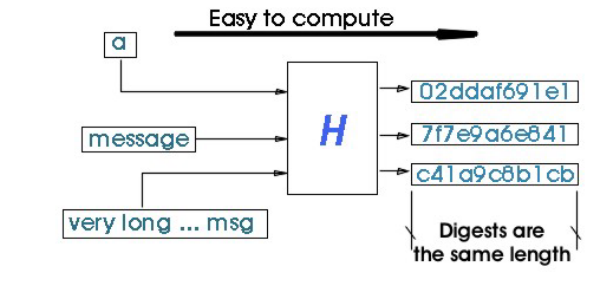
\includegraphics[width=0.5\textwidth]{images/hash_function.png}
%   \caption[Components of Bitcoin block]{Components of Bitcoin block}
%   \label{fig:hash_function}
% \end{figure}

% The fomular is:
% \begin{align*}
%   h & = H(M) \\ \intertext{ Where h is hash value, M is pre-image and H is cryptographic hash function.}
% \end{align*}


% According to NIST, a cryptographic hash mush satisfied following three properties:
% \begin{enumerate}
%   \item Collision resistance: It is computationally infeasible to find two inputs that have the same hash value.
%         The most efficient method to find must be brute-forcing of random inputs.
%         \emph{The birthday "paradox"} places an upper bound on collision resistance.
%         That is, the complexity (or collision-resistance strength) of seeking two different input \emph{M} and \emph{M'} matched two hash \emph{H(x)} = \emph{H(x’)} equal to \emph{L/2} bit-operations for a \emph{L-bit} hash function.
%         For example, SHA-512 produces a collision resistance of 256 bits.

%   \item Pre-image resistance: Given a hash value \emph{h}, it is computationally infeasible to find an M that \emph{H(M)=h}.
%         Preimage resistance strength is equal to the amount of work to brute-force \emph{L-bit} of operations for a \emph{L-bit} hash function.
%         For example, SHA-512 provides a preimage resistance of 512 bits.

%   \item Second pre-image resistance: Finding a second input that has the same hash value as any other specified input would be computationally infeasible.
%         Second preimage resistance is calculated by the number of operations equal to  \emph{L} bits for a \emph{L-bit} hash function.
%         For example, SHA-512 produces a (full-length) hash value of 512 bits.
%         However, in some cases of the hash functions, the second preimage resistance also depends on the length of the message resulting from the hash function.

% \end{enumerate}

% \subsubsection{Choosing Approved Hashs}
% NIST approved following algorithms:
% \begin{itemize}
%   \item SHA-1 \cite{DBLP:journals/cryptologia/Dang13}

%   \item SHA-2 family: SHA-224, SHA-256, SHA-384, SHA-512, SHA-512/224, and SHA-512/256. \cite{DBLP:journals/cryptologia/Dang13}

%   \item SHA-3 family (on KECCAK \cite{DBLP:journals/iacr/BertoniDPA15} as a result of the “SHA-3” Cryptographic Hash Algorithm Competition):  SHA3-224, SHA3-256, SHA3-384, SHA3-512, SHAKE128 and SHAKE256.
% \end{itemize}
% Due to the fact that SHA-1 already has a collision \cite{SHA-1:Collision}, we won't choose SHA-1 for usage in our thesis.
% Considering the blockchain system we working on, the hash algorithm will be choose in the future.

% \bigskip
% {\textit {\textbf{Best Known attacks on Hash function}}}

% \subsection{Asymmetric-key cryptography}
% \label{sec:asymmetric_cryptography}
% Asymmetric-key cryptography, or Public-key cryptography required a related pair of keys: a public key and a private key to form a cryptographic system.
% The public key is known by anyone while the private key is kept secret. Our thesis apply assymmetric-key cryptography in authentication, confidentiality and exchange \emph{\hyperref[sec: Symmetric_keys]{symmetric key}}.
% In this chapter, we will introduce various algorithms of public-key cryptography and chooing the best one for final project.

% \subsubsection{Asymmetric encryption}
% To perform asymetric encryption/decryption, each users have to generate a public-private key pair.
% Data can be encrypted with the public key and decrypted with the private key.

% \begin{figure}[ht!]
%   \centering
%   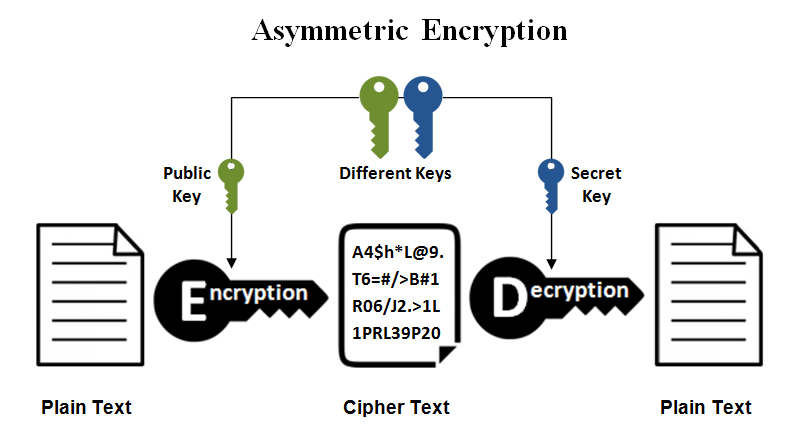
\includegraphics[width=0.5\textwidth]{images/asymmetric_encrypt.png}
%   \caption[Model of asymmetric encryption and decryption]{Model of asymmetric encryption and decryption}
%   \label{fig:asymmetric_encrypt}
% \end{figure}

% \subsubsection{Diffie-Hellman algorithm - A key agreement protocol}
% Diffie-Hellman is one of the first public-key protocols named after Whitfield Diffie and Martin Hellman the creators.
% Today DH algorithm is used across the Internet.
% Making use of the speed of Symmetric-key cryptography, DH supports users and servers can exchange private key on an non-secure channel.
% In our thesis, DH algorithm play an important role in TLS 1.3.

% \bigskip
% {\textit {\textbf{Math behind Diffie-Hellman algorithm}}}

% The DH protocol uses multiplicative group of integer modulo $p$ and $g$ is a primitive root modulo $p$.
% p is a big prime number.
% Assume Alice and Bob want to share the same key, they follow these steps:
% \begin{enumerate}
%   \item Alice and Bob agree on a finite cyclic group $G$ of order $n$ and a generating element $g$ in $G$.
%         \begin{definition}
%           Cyclic group (aka. monogenous group) is a group that generated by the generator.
%         \end{definition}
%   \item Alice choose a random natural number $a$, where $1 < a < n$ then sends $g^a$ mod $n$ to Bob.
%   \item Bob do the same with random natural number $b$ and sends $g^b$ mod $n$ to Alice.
%   \item Alice calculate $(g^b \, mod \, n)^a$ mod $n$
%   \item Bob calculate $(g^a \, mod \, n)^b$ mod $n$
% \end{enumerate}
% Now Alice and Bob possessed the same private key $g^ab$ mod n.
% Our thesis use DH algorithm as minor part in TLS 1.3.
% Later if we have enough time to actually made a product, we will need TLS 1.3 for connection between Wallet and the Blockchain network.
% So if everything go as planned, we are going to mentioned further DH base algorithm.

% \subsubsection{DSA - Digital Signature Algorithm}
% Data, in our case, transaction sent through the blockchain network requires some digital signing mechanisms to prove authenticity of the sender.
% The Digital Signature Algorithm provides methods of generating a digital signature and verifying validity of the signature.
% Everytime we create a transaction, we digitally signing a transaction (for example says "I'm sending 1 SOL to this guy address) then sent to other nodes on the network.
% They can check that your signature matches the message. If it doesn’t, they’ll just reject it.
% A digital signature is like a 'fingerprint' or a written signature of the owner in electronic world.
% It also provides integrity of transactions (i.e detect if the transaction was tampered after it was signed) and non-repudiation.

% \begin{figure}[ht!]
%   \centering
%   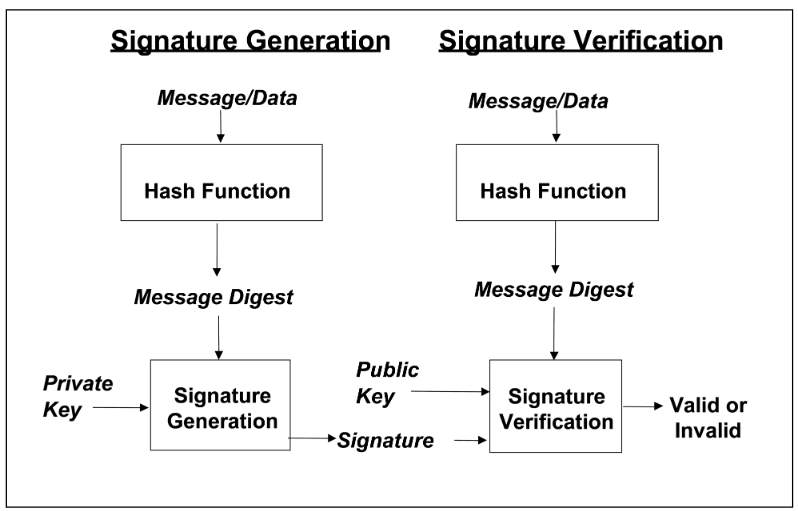
\includegraphics[width=0.8\textwidth]{images/digital_signature.png}
%   \caption[Digital signature process]{Digital signature process}
%   \label{fig:digital_signature}
% \end{figure}

% The Digital Signature Algorithm was proposed in August 1991 by NIST and released in Digital Signature Standard \cite{DSS1998}, but no longer approved in the latest Digital Signature Standard Document \cite{DSS2019}.
% Thus, we won't dive deep into the DSA but only the process scheme of electronically signing and verifying a signature since all Cryptographic signature algorithms will follow this standard.
% In this section, we have the idea of how digital signature works.

% \subsubsection{RSA Cryptography}

% RSA is the oldest public-key cryptosystem. The acronym RSA comes from the surnames of Ron Rivest, Adi Shamir and Leonard Adleman, who publicly described the algorithm in 1977. The RSA algorithm requires selecting two large prime numbers to generate a pair of public key and private key. The primes and the private key are kept secret, while the multiplication of two primes and the public key are visible. This way, the messages can be encrypted by anyone but can only be decrypted by the owner of the corresponding private key.

% The RSA algorithm involves four steps: key generation, key distribution, encryption and decryption. To generate a pair of valid keys:

% \begin{enumerate}
%   \item Choose two distinct primes number $p$ and $q$.
%   \item Compute $n = p \times q$ and $\phi(n) = (p - 1)(q - 1)$, where $\phi$ is called Euler's totient function
%   \item Choose an integer $e$ such that $1 < e < \phi(n)$ and $e$ must be coprime with $\phi(n)$ and $n$
%   \item Determine an integer $d$ satisfied the equation $d \equiv e^{-1}\ (\textrm{mod}\ \phi(n))$; where $d$ is the modular multiplicative inverse of $e$ modulo $\phi(n)$, means that $de \equiv 1\ (\textrm{mod}\ \phi(n))$.
% \end{enumerate}

% The public key consists of the modulus $n$ and the exponent $e$. The private key is the exponent $d$, which must be kept secret, the same goes to $p$ and $q$ since they can be used to calculate $d$. In fact, $p$ and $q$ can be discarded after $d$ has been computed. To distribute the public key, the user simply sends it via a reliable, but not necessarily secret, route. For the encryption/decryption scheme, suppose that Bob wants to send Alice a message $m$, and Bob has already got Alice public key. Bob encrypts the message using the equation:

% \begin{equation}
%   m^e\ \equiv\ c\ (\textrm{mod}\ n)
% \end{equation}

% The cipher text $c$ is the result of the encrypted message. Bob then transmits $c$ to Alice. When Alice got $c$, she can decrypt the cipher text as follow:

% \begin{equation}
%   c^d\ \equiv\ (m^e)^d\ \equiv\ m^{ed}\ \equiv\ m^1\ \equiv m\ (\textrm{mod}\ n)
% \end{equation}

% Notice that thorough the action, we only use Alice' keys. Alice's public key acts as an address of where to send the message to, and her private acts as a key to her mailbox, only she can open and read what the message is. RSA also comes with a digital signature scheme, which is reversely included only Bob' keys: Bob will use his private key to sign the message, and the signature can be verify by Alice using the public key of Bob. Suppose that Alice wants to know if the message is exactly come from Bob and Bob wants to clarify that. Bob first hashes the message using a hash function, denoted $h = H(m)$. Then he signs the message using his private key:

% \begin{equation}
%   h^d\ \equiv\ s\ (\textrm{mod}\ n)
% \end{equation}

% Attached the signature $s$ to the message, Bob sends them to Alice (of course, after encrypted as described above). To verify a signature $s'$ is Bob signature $s$, Alice verifies $s$ by comparing $h'$ and $h$ where $h'$ is retrieved from:

% \begin{equation}
%   (s')^e\ \equiv\ ((h')^d)^e\ \equiv\ (h')^{de}\ \equiv\ h'\ (\textrm{mod}\ n)
% \end{equation}

% If $h' = h$ then $s' = s$, the signature is valid and Bob is the sender of the message. This scheme works because of $de \equiv 1\ (\textrm{mod}\ \phi(n))$ and exponentiation rules:

% \begin{equation}
%   (h^d)^e\ \equiv\ h^{de}\ \equiv\ h^{ed}\ \equiv\ (h^e)^d \equiv\ h \ (\textrm{mod}\ n)
% \end{equation}

% The security of RSA algorithm depends on the integer factorization problems, where we can easily multiply two distinct primes, but it's hard to retrieve two primes from the multiplication. This is called one-way function (or trapdoor function), the backbone of the asymmetric cryptography. Because the encryption key is public, we need to ensure that neither the public key nor the encryption reveals anything about the private key and the decryption. It's easy and fast to encrypt, but it's hard and infeasible to decrypt without knowing the private key. By relying on the integer factorization, RSA is simple and effective for a long time until the computing power becomes so strong nowadays and even parallelism. That where the weakness of RSA comes in: the complexity of RSA doesn't grow exponential when increasing the number. It causes the size of keys are becoming larger if we want to be more secure. The larger the number is, the slower the decryption runs. Therefore; ECC has gradually gain more attention in terms of secure and cost-efficient.

% \subsubsection{ECC - Elliptic Curve Cryptography}
% \begin{definition} (Abelian Group) 
%   A group G with the binary operation (.) is said to be {\bf abelian} if it satisfies the commutative condition $( \forall  \, a,b \, \in G,  \, a . b  \, =  \, b . a )$.
% \end{definition}

% \begin{figure}[ht!]
%   \centering
%   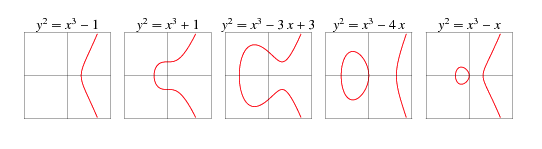
\includegraphics[width=1\textwidth]{images/example_curve.png}
%   \caption[Elliptic Curve Example]{Elliptic Curve Example}
%   \label{fig:ec_example}
% \end{figure}

% Proposed by Neil Koblitz and Victor Miller in 1985, \emph{Elliptic Curve Cryptography} is a more powerful alternative approach to \emph{RSA}. \emph{ECC} offers a faster, less computational energy in crypto-progress, higher security and shorter key pairs.
% An elliptic curve is a two-space graph defined by the square roots of a cubic equation. In cryptography, it takes a form defined as follows

% \begin{equation}
%   \emph{E} = \{{O}\cup{(x,y)\in \mathbb{F}_{p}^2 \,|\, y^2 = x^3 + ax + b, \, 4a^3 + 27b^2 \neq 0}\}
% \end{equation}

% where (\emph{a,b}) $\in\mathbb{F}_{p}^2$ and O is the point at infinity which is considered to be the neutral element of the curve. The condition $4a^3 + 27b^2 \neq 0$ make the curve not singular since it will be isomorphic to multiplicative group, which enables to solve DLP faster [Singular curve attack]. Singular curves may have a cusp or multiple roots (\autoref{fig:singularities}).

% \begin{figure}[ht!]
%   \centering
%   
\includegraphics[width=0.3\textwidth]{images/singularities.png}
%   \caption[Invalid curves]{Invalid curves}
%   \label{fig:singularities}
% \end{figure}

% This is referred to as the Weierstrass equation for an elliptic curve.
% \autoref{fig:ec_example} show some examples of elliptic curve shaping different forms depend on a and b.
% Denoted by E($\mathbb{F}_{p}^2$) the elliptic curve over the finite field $\mathbb{F}_{p}^2$.
% Because elliptic curve over $\mathbb{F}_{p}^2$ still construct a abelian group, for general purposes, we won't mention the standard line equation for $\mathbb{F}_{p}$ (mod p in the end of the equation).


% {\textit {\textbf{The Group Law}}}

% Examine adding point on curve (\autoref{fig:ec_example}), we can see the process work as follow:
% \begin{figure}[ht!]
%   \centering
%   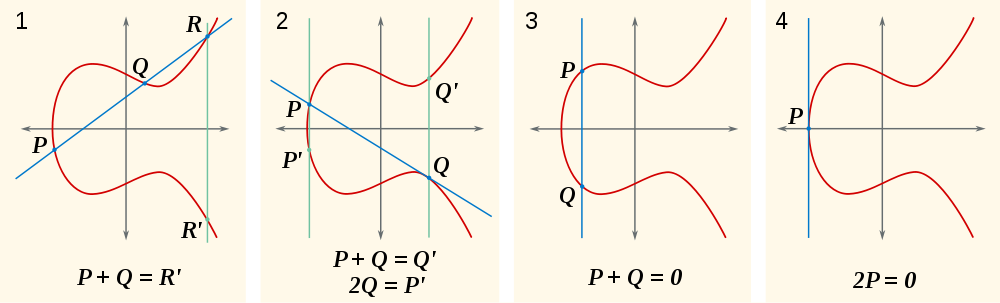
\includegraphics[width=1\textwidth]{images/adding_point.png}
%   \caption[Adding point on elliptic curve]{Adding point on elliptic curve}
%   \label{fig:add_point}
% \end{figure}
% \begin{itemize}
%   \item For each point P on the curve E($\mathbb{F}_{p}^2$), the point at infinity (O) serves as the identity element, i.e., P + O = O + P = P.
%   \item For each point P = (x, y) on the curve E($\mathbb{F}_{p}^2$), the point -P is the point (x, -y) and has P + (-P) = O.
%   \item Let $P_1 =(x_1, y_1)$ and $P_2 = (x_2, y_2)$ be points on the curve E($\mathbb{F}_{p}^2$), where $P_1 \neq \pm P_2$, let $Q = P_1 + P_2$. Then Q = (x, y) where  \medskip
%         \begin{align*}
%           x + x_1 + x_2 = \lambda^2 and y + y_1 = \lambda(x_1 - x), \,	where \, \lambda = (y_2 - y_1)/(x_2 - x_1). \\
%         \end{align*}
%   \item Let $P = (x_1, y_1)$ be a point on the curve E($\mathbb{F}_{p}^2$), where $P \neq -P$, and let $Q = 2P$. Then $Q = (x, y)$, where \medskip
%         \begin{align*}
%           x + 2x_1 = \lambda^2 \, and \, \, y + y_1 = \lambda(x_1 - x), \, where \, \lambda = (3x_1^2 + a)/2y_1
%         \end{align*}
%   \item For a point P on E($\mathbb{F}_{p}^2$), a positive integer k, we define the multiplication as: \medskip
%         \begin{align*}
%           kP = \underbrace{P + P + P ... + P}_\text{k}. \\
%         \end{align*}
%         Where k is negative, we use
%         \begin{align*}
%           kP = -k(-P). \\
%         \end{align*}
% \end{itemize}
% Every point P on E($\mathbb{F}_{p}^2$) exists a non-negative integer \emph{k} such that $kP = O$. In this case, the smallest \emph{k} is the {\bf order} of the P on E.

% \bigskip
% {\textit {\textbf{Order of an elliptic curve group}}}

% We mentioned curve over finite fields $\mathbb{F}_{p}$. So it must have finite number of points.
% The {\bf order} of a group is the number of points belong to that group.
% In practice, we need to know the minimum size of a elliptic curve to prevent certain brute-force attack.
% Applying Hasse's algorithm \cite{hasse}, order of the curve bound to a range:\medskip
% \begin{align*}
%   p + 1 - 2\sqrt{p} \leq order(E) \leq p + 1 + 2\sqrt{p}
% \end{align*}

% \bigskip
% {\textit {\textbf{Cyclic subgroup of elliptic curve}}}
% \begin{figure}[ht!]
%   \centering
%   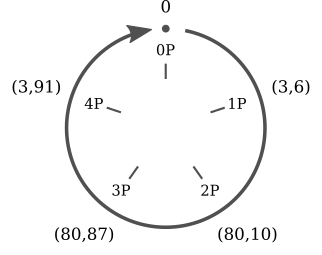
\includegraphics[width=0.5\textwidth]{images/cyclic_ec.png}
%   \caption[Example curve $y^3=x^3+2x+3$]{Example curve $y^3=x^3+2x+3$ over $\mathbb{F}_{97}$}
%   \label{fig:cyclic_ec}
% \end{figure}

% Observing multiple addition of point \emph{P}, we can spot the results are repeating cyclically.
% These multiples of \emph{P} is a cyclic subgroup of the group created by elliptic curve.
% The point \emph{P} will generate the whole group by repeating operation "$+$" multiple times.
% Then \emph{P} is the generator (a.k.a. base point) of the cyclic group.

% The order of cyclic group is the smallest number \emph{n} such that $nP = O$ (O is the point at infinity).
% \emph{Lagrange's theorem} states that the order of a subgroup is a divisor of the order of the parent group.
% In our case, \emph{n} is a divisor of \emph{N}, where \emph{N} is number of points of a elliptic curve.
% If \emph{N} is a prime then $n = N$.
% For cryptographic application, \emph{n} has to be a prime otherwise the cyclic group will be vulnerable to the attacks using \href{https://crypto.stanford.edu/pbc/notes/numbertheory/crt.html}{Chinese Remainder Theorem}.
% \autoref{fig:cyclic_ec} shows an example of a cyclic group of 5 elements with the base point $P = (3,6)$.
% We also have $5P = O$.

% % "With anything that forms a cyclic group, we can create a cryptographic system base on it" - Christopher Parr. 
% \bigskip
% {\textit {\textbf{Elliptic Curve Discrete Logarithm Problem (ECDLP)}}}
% \begin{definition}
%   Given an elliptic curve \emph{E}. We consider a primitive element P and another T. The Discrete Logarithm problem is finding the integer d, where 1 $\leq$ d $\leq$ order(E), such that: \medskip
%   \begin{align*}
%     \underbrace{P + P + P ... + P}_\text{d times} = dP = T \\
%   \end{align*}
% \end{definition}

% This problem is "discrete" because it involves cyclic groups, it is "logarithm" since it's analogous to ordinary logarithms \cite{dlp}.
% In our cryptosystems, the integer \emph{d} will be chosen as the private key while \emph{T = (x,y)} is an element of curve E with generator be the public key.
% The Discrete Logarithm problem here is how "hard" to find \emph{d} given $P$ and $T$.
% There beliefs that no such polynomial time algorithm could solve this problem.
% The best known algorithm is The Square Root attacks that cost about $\sqrt{d}$ computations.
% If $d$ is a big prime with the length of 256 bits, it would cost $\sqrt{d} = \sqrt{2^{256}} = 2^{128}$ steps to find $d$.
% $2^{128}$ is more than number of molecules on Earth.
% Comlplexity of this problem can't be solved using classical computer.
% Every cryptosystems these day are dependent on ECDLP.
% If everyone can break ECDLP, cryptosystems will collapse.

% \bigskip
% {\textit {\textbf{Security level of ECC vs RSA}}}

% Modern systems are migrating from RSA Cryptography to ECC type due to fact that EC provided the same security level as RSA with smaller key size.
% Latest handshake protocol TLS 1.3 (which supports all Fintech wallet (MoMo, ZaloPay...), Website, and IoT systems) completely remove RSA and using EC in all steps.
% \autoref{fig:ecc_security_level} is a comparision of EC vs RSA.

% \begin{figure}[ht!]
%   \centering
%   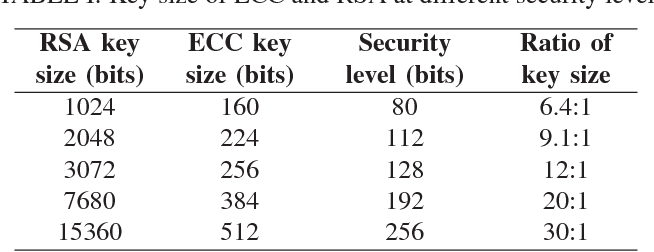
\includegraphics[width=0.7\textwidth]{images/ecc_security_level.png}
%   \caption[EC vs RSA]{Same security level comparision}
%   \label{fig:ecc_security_level}
% \end{figure}

% \bigskip
% {\textit {\textbf{Elliptic Curve Digital Signature Algorithm}}}

% Assuming Alice want to send some coins to Bob. First of all they have to agree on a \emph{safe curve} \cite{nist_safe_curve}.
% Domain parameter is already set up and include:
% \begin{itemize}
%   \item Curve $E$
%   \item Base point G
%   \item Order n of subgroup generated by G (n must be large prime)
%   \item Recommended Hash function (HASH) \cite{SHS2015}
%         \begin{quote}
%           Security level of chosen hash function is big problem in ECDSA, NIST did approved some of the hash algorithm we mentioned in Section~\ref{sec:crypto_hash}.
%           For example, if hash function has weak second-image resistance, attackers who sniffing between can modify the transaction and the signature will remain the same.
%           This may lead to hugh consequences.
%           In our thesis, we only use SHA-2 or SHA-3 families to make certain we won't be a vulnerable object to these type of attacks. These attacks are passive Man-In-The-Middle (MITM) attacks, we need TLS to prevent active MITM attacks.
%         \end{quote}
% \end{itemize}

% Alice need to create a {\bf random generate} private key $d_A$ between $[1, n-1]$ and calculate public key $Q_A = d_An$.
% For certain kinds of attacks, ANSIX9.62 recommended the length of keys at least 160 bits.
% To sign a transaction $m$, Alice will do:
% \begin{enumerate}
%   \item Calculate $Hash(m)$ and convert this bit string to integer $z$.
%   \item Create a random integer $k$ using Cryptographic Random, $k$ in range [1, n-1]. $k$ is kept secret and $k$ is per message or transaction.
%   \item Compute $kG = (x_1, y_1) \in E$.
%   \item Compute $r=x_1$ mod n. If $r = 0$ go back to step 2.
%   \item Compute $s=k^{-1}(z + rd_A)$ mod n. If $s = 0$ go back to step 2.
%   \item $m'$ is the signature for the transaction m with $m' = (r, s)$.
% \end{enumerate}
% The process above is called ECDSA Signature Generation.
% Weak random k is also vulnerable to some kind of attacks.
% Cryptographic random algorithm play a extremely important row in cryptosystems like Crypto Wallet and SSL/TLS.
% For example, failure in number generation cause thefts to steal user private keys.
% In 2013, Edward Snowden published information about random-generator-base backdoor that NSA put into communication system to spoofing messages (\href{https://www.bbc.com/news/technology-24048343}{NSA backdoor}).

% Now Bob has to verify Alice's signature. ECDSA Signature Verification contains following step:
% \begin{enumerate}
%   \item Verify $Q_A$ is a valid point lies on $E$ (not equal $O$).
%   \item Verify if $nQ_A = O$.
%   \item Verify if $r$, $s$ are integer in [1, n-1].
%   \item Compute $Hash(m)$ and convert this bit string to an integer $z$.
%   \item Compute $u_1=zs^{-1}$ mod n and $u_2= rs^{-1}$ mod n.
%   \item Compute $X = u_1G + u_2Q_A = (x_1, y_1)$.
%   \item Check if $X = O$ then the signature is invalid.
%   \item Check if $r = x_1$ then the signature is valid, otherwise return invalid.
% \end{enumerate}

% {\textbf{Proof of Correctness}}

% $u_1G + u_2Q_A = zs^{-1}G + rs^{-1}d_AG = s^{-1}(z+d_Ar)G =(k^{-1})^{-1}(z+d_Ar)^{-1}(z+d_Ar)G = kG$

% \bigskip
% {\textit {\textbf{Best Known attacks on ECC}}}

% \subsection{Twisted Edward Curve and ed25519}
% The twisted Edward curve was obtained form the Montgomery curve via an isomorphic mapping.
% Taking the form $x^2 + y^2 = c^2(1+ x^2y^2)$ over the non-binary field $k$.
% We will cover this part in our thesis as the main part.

% \subsection{Child key derivation function}
% Key derivation play a huge role in HD wallet.
% Bips32 of Bitcoin wallet did a huge favor for cryptocurrencies because of creating such magnificient function.
% This function helps users, web server to calculate the public keys of the recievers without the access to private key.
% Our thesis aim to create a Child key derivation function for Twisted Edward Curve.
% We will mention this again in our thesis report.

% \subsection{Symmetric-key cryptography}
% \label{sec: Symmetric_keys}
% Usage: In TLS

% \subsubsection{TLS 1.3}
% Usage: Secure connection


